\documentclass[../review_1.tex]{subfiles}
\graphicspath{{\subfix{../img/}}}
\begin{document}

\chapter{Vorgehen}\thispagestyle{fancy}
\section{Vorgehensmodell und die Anpassung des Vorgehens}
% damit ist v. a. die Anpassung an den Unified Process als Vorgehensmodell gemeint
Ein Vorgehensmodell legt einen bestimmten Ansatz für die Art der Durchführung und die Reihenfolge der Teilaufgaben der Systementwicklung maßgeblich fest. Erst mit einem Vorgehensmodell wird ein komplexer Softwareentwicklungsprozess übersichtlich, plan- und strukturierbar. Die Wahl des Vorgehensmodells ist deshalb von enormer Bedeutung.\\
Im \textbf{Wasserfallmodell} sind zwar Planung, Kontrolle und Steuerung vergleichsweise einfach, jedoch erfordern Rücksprünge einen hohen Änderungsaufwand in allen Dokumenten. Somit zeigt sich dieses sequentielle Modell unflexibel gegenüber Projekten, bei denen sich die Anforderungen an das zu entwickelnde Projekt oft verändern. Dies ist jedoch hier, da durch die Komplexität des Themas eventuell erst einige Anforderungen später identifiziert werden. \\
Es wurde gegen ein \textbf{agiles Vorgehen} gestimmt, da unter anderem das Projektmanagement in diesem Vorgehensmodell durch das chaotische Vorgehen sehr schwierig ist. Außerdem hat die Planbarkeit des Ergebnisse hohe Priorität.\\
Letztlich wurde sich für den \textbf{Unified Process} (siehe Abb. \ref{up}) entschieden. Dieses Vorgehensmodell nutzt die UML als Notationssprache.
\vspace{-0.3cm}
\begin{figure} [h]
    \centering
    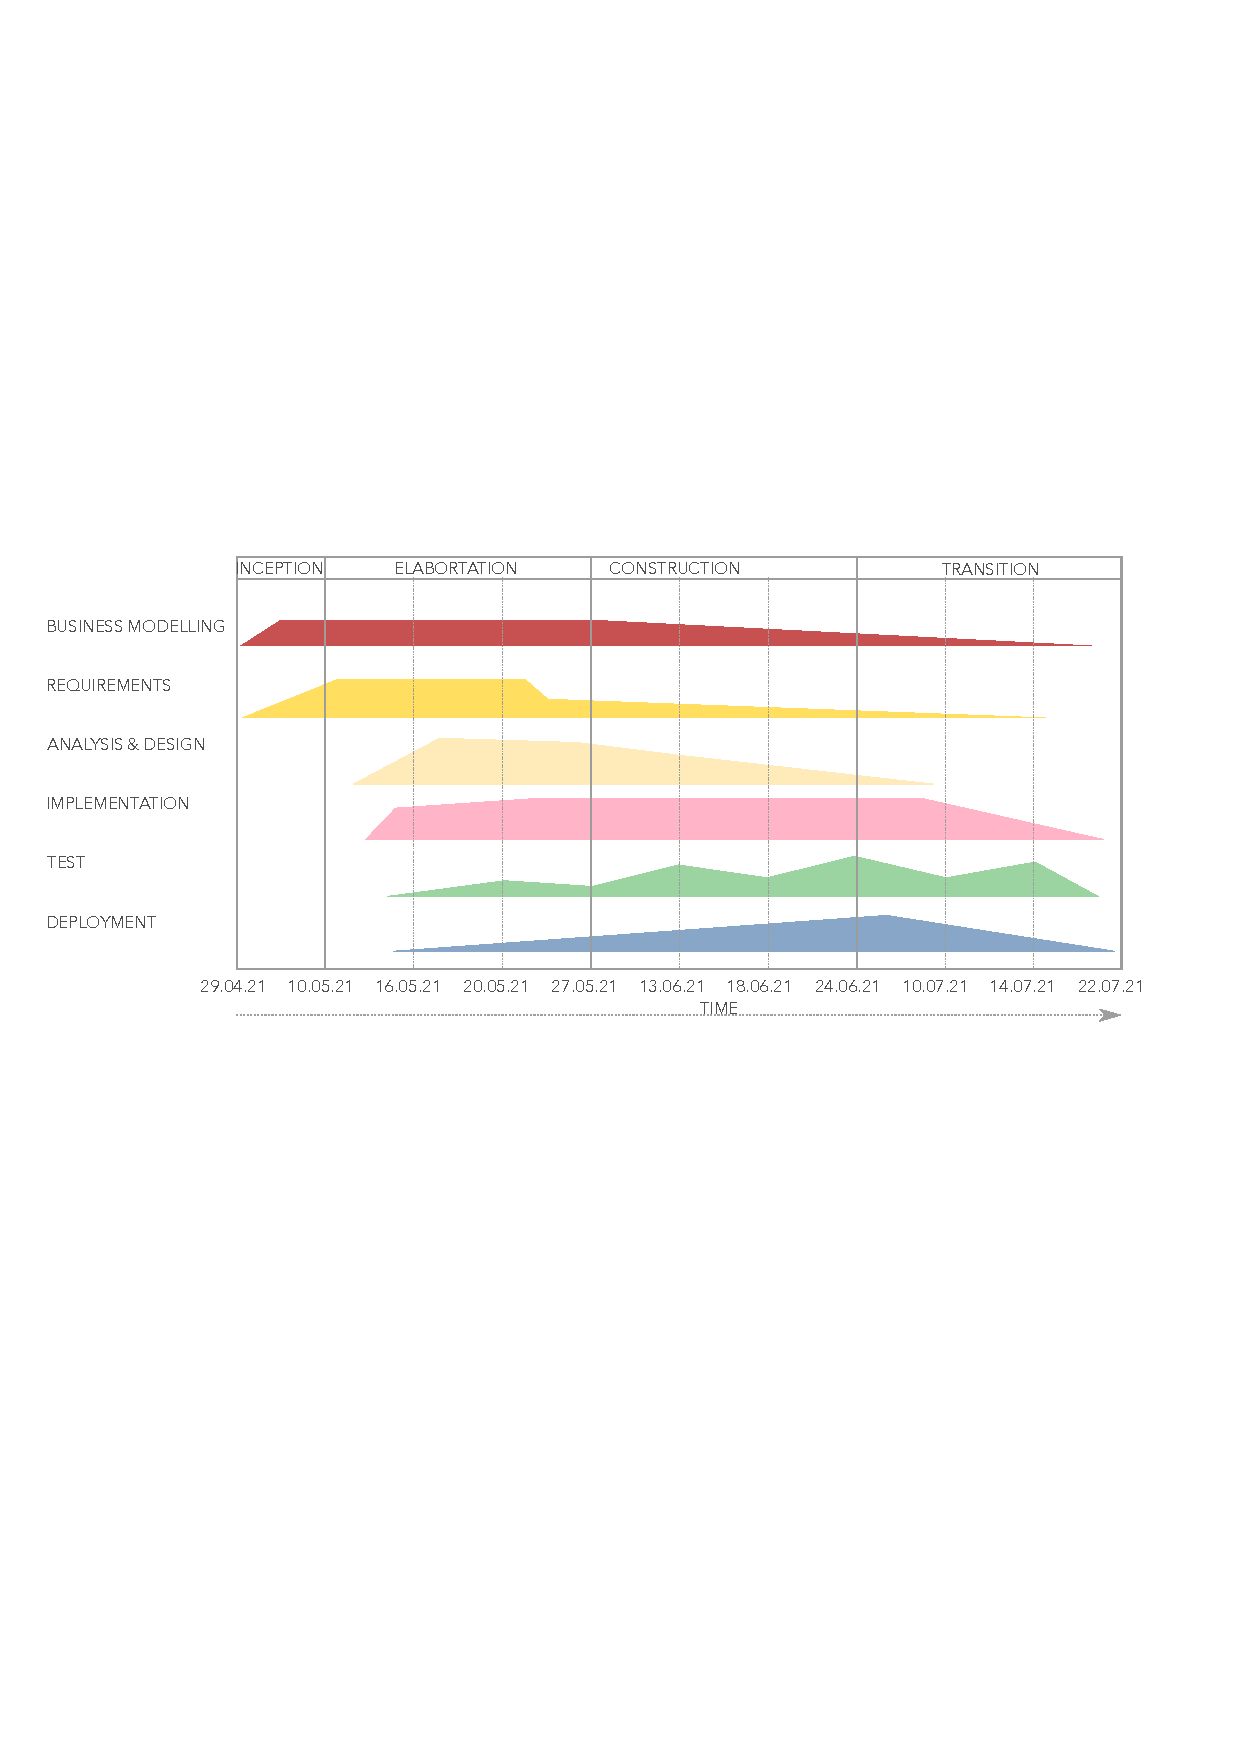
\includegraphics[height = 6.5cm]{UnifiedProcess.pdf}
    \caption{Angepasstes Vorgehensmodell (Unified Process)}
    \label{up}
\end{figure}
\\ \newline Grundsätzlich besteht dieses iterative und inkrementelle Vorgehensmodell aus vier Phasen. Zu Beginn des Projekts werden in der \textbf{Konzeptionsphase} (inception phase) die zentralen Anforderungen ermittelt, der Projektumfang definiert und möglichst viele Projektrisiken entdeckt. Diese Phase stellt die Kürzeste dar. Sie endet mit dem Milestone lifecycle objective.\\
Auf die Konzeptionsphase folgt die \textbf{Ausarbeitungsphase} (elaboration phase), in der unter anderem die Systemanforderungen vervollständigt und die Entwurfsspezifikation entwickelt werden. Hier wird auch ein erster Protoptyp erarbeitet. In diesem Projekt umfasst diese Phase sowohl den Entwurf, als auch große Teile der Planung. Diese Phase besteht aus drei Iteration, wobei die Iterationen unterschiedlich lange sind. In jeder Iteration wird das vorherige Ergebnis verfeinert.	\\
In der \textbf{Konstruktionsphase} (construction phase) findet ein Großteil der Implementierung, aber auch des Testens statt.\\
Die letzte Phase ist die \textbf{Inbetriebnahme} (transition phase). Die Auslieferung der Software an den Kunden wird im vorliegenden Projekt sehr kurz ausfallen. Jedoch wird in dieser Phase zusätzlich verstärkt getestet.\\
In den Phasen laufen verschiedene Kernprozesse zu unterschiedlichen Anteilen parallel ab. Man kann die einzelnen Phasen wie folgt ins Deutsche übersetzen: Business Modelling $\widehat{=}$ Geschäftsprozessmodellierung, Requirements $\widehat{=}$Anforderungsanalyse, Analysis and Design $\widehat{=}$ Analyse und Design, Implementation $\widehat{=}$ Implementierung, Test $\widehat{=}$ Test, Developmenent $\widehat{=}$ Auslieferung. \\
Aus dem agilen Vorgehen wurden für das Projekt einige Prinzipien übernommen: Zum einen die \textbf{häufigen Meetings} und \textbf{kurzen Statusmeldungen}, damit jedes Teammitglied genau weiß, wo die anderen Mitglieder stehen und was deren derzeitigen Probleme sind.\\
Zudem ist durch Gitlab ein \textbf{Kanbanboard} (siehe Abb. \ref{board}) verfügbar. Mit diesem agilen Projektmanagement-Tool werden die Aufgaben visualisiert. Es hilft dem Projektteam, die Arbeit zu strukturieren und so deren Effizienz zu steigern.\\
\vspace{-0.5cm}
\begin{figure} [h]
    \centering
    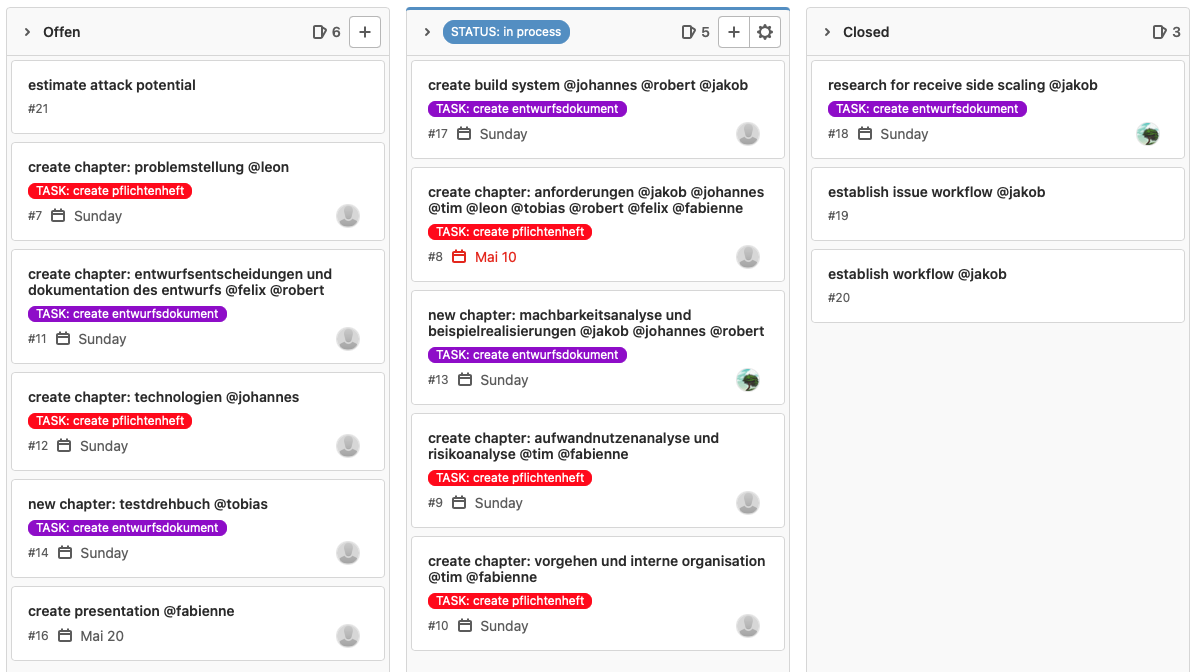
\includegraphics[height = 8cm]{kanban.png}
    \caption{Board auf Gitlab (Datum des Screenshots: 15.05.2021)}
    \label{board}
\end{figure} \\
\noindent Auch wurde sich innerhalb des Projektteams auf (agile) \textbf{Werte} geeinigt, um eine bestmögliche Zusammenarbeit zu gewährleisten (siehe Abb. \ref{werte}).
\begin{figure} [H]
    \centering
    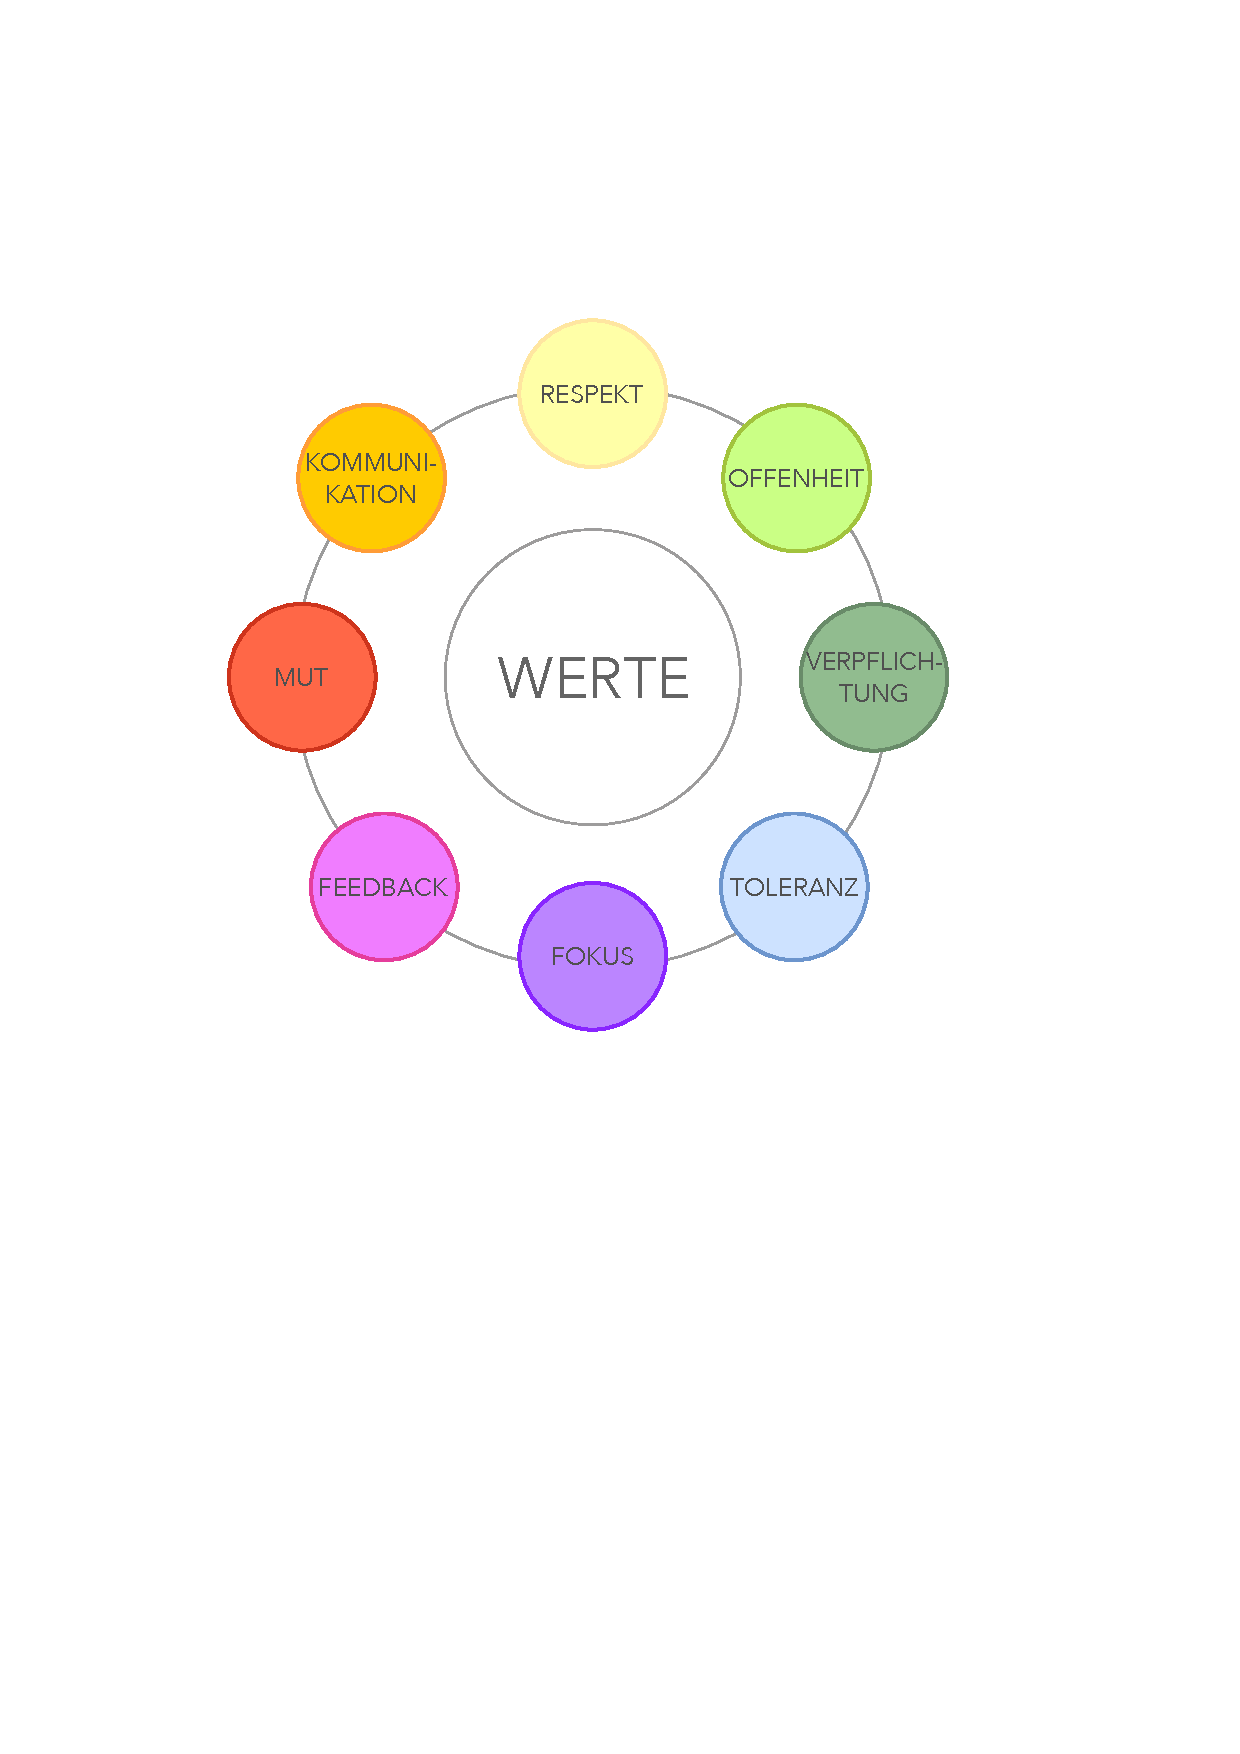
\includegraphics[height = 5cm]{Werte.pdf}
    \caption{Werte}
    \label{werte}
\end{figure}
Jedes Teammitglied zeigt \textbf{Respekt} gegenüber die anderen und schätzt diese. Außerdem zeigen es jedem Verständnis, wenn beispielsweise jemand ein Problem hat. Zudem wird auch auf die Schwächeren Rücksicht genommen.\\
\textbf{Offenheit} bedeutet hier, dass neue Informationen und Erfahrungen bewusst aufgenommen werden und nicht vorschnell als unwichtig bewertet werden. Jeder darf seine Meinung frei äußern, um Missverständnissen und Auseinandersetzungen vorzubeugen. Ebenso soll Transparenz herrschen und Problemen sollen sofort auf den Grund gegangen werden. \\
Der Wert \textbf{Verpflichtung} kann so interpretiert werden, dass alle Teammitglieder sich der Projektaufgabe verbunden fühlen sollen.\\
Außerdem sind \textbf{Toleranz} und Vielfalt zentrale Werte. Personen mit anderen Sichtweisen werden nicht etwa als Konkurrenten gesehen, sondern vielmehr als Bereicherung für das Team.\\
Der \textbf{Fokus} liegt im Projekt vor allem auf den Aufgaben und auf den gemeinsamen Zielen. Verschwenden von Zeit und Kapazitäten und Ablenkungen sollen vermieden werden. Zudem hat die Fertigstellung einer bereits begonnen Aufgabe Vorrang gegenüber den Start einer neuen Aufgabe.\\
Indem in den Meetings regelmäßig der derzeitige Stand aufgezeigt wird, kann sich jedes Teammitglied individuelles \textbf{Feedback} von den anderen Beteiligten holen.\\
Zusätzlich soll jedes Teammitglied \textbf{Mut} aufweisen, indem es zum Beispiel neue Aufgaben übernimmt, die vielleicht zuerst als schwer machbar und komplex erscheinen. Außerdem erfordert es Mut zu sagen, wenn man Hilfe benötigt, aber auch mitzuteilen, dass man hinter dem Zeitplan liegt. Auch das Ausprobieren neuer Lösungswege fällt unter den Wert Mut.\\
Zudem ist die tägliche \textbf{Kommunikation} mit den Teammitgliedern für eine gute Zusammenarbeit erforderlich. So sollte jeder beispielsweise mehrmals täglich nach neuen Zulip-Nachrichten schauen und dort auf Fragen antworten. Außerdem wurde gemeinsam beschlossen, dass man bei Änderungen an den Dokumenten andere benachrichtigt.

\section{Projektplan}
Der Projektplan besteht aus verschiedenen Objekten: Dem Projektstrukturplan und einem Ablaufplan (hier Gantt-Diagramm).\\
Der \textbf{Projektstrukturplan}, welcher in Abb. \ref{projektstrukturplan} zu sehen ist, gliedert und strukturiert das Projekt hierarchisch. Er ist die Grundlage für die Ablaufplanung. 
\begin{figure} [h]
    \centering
    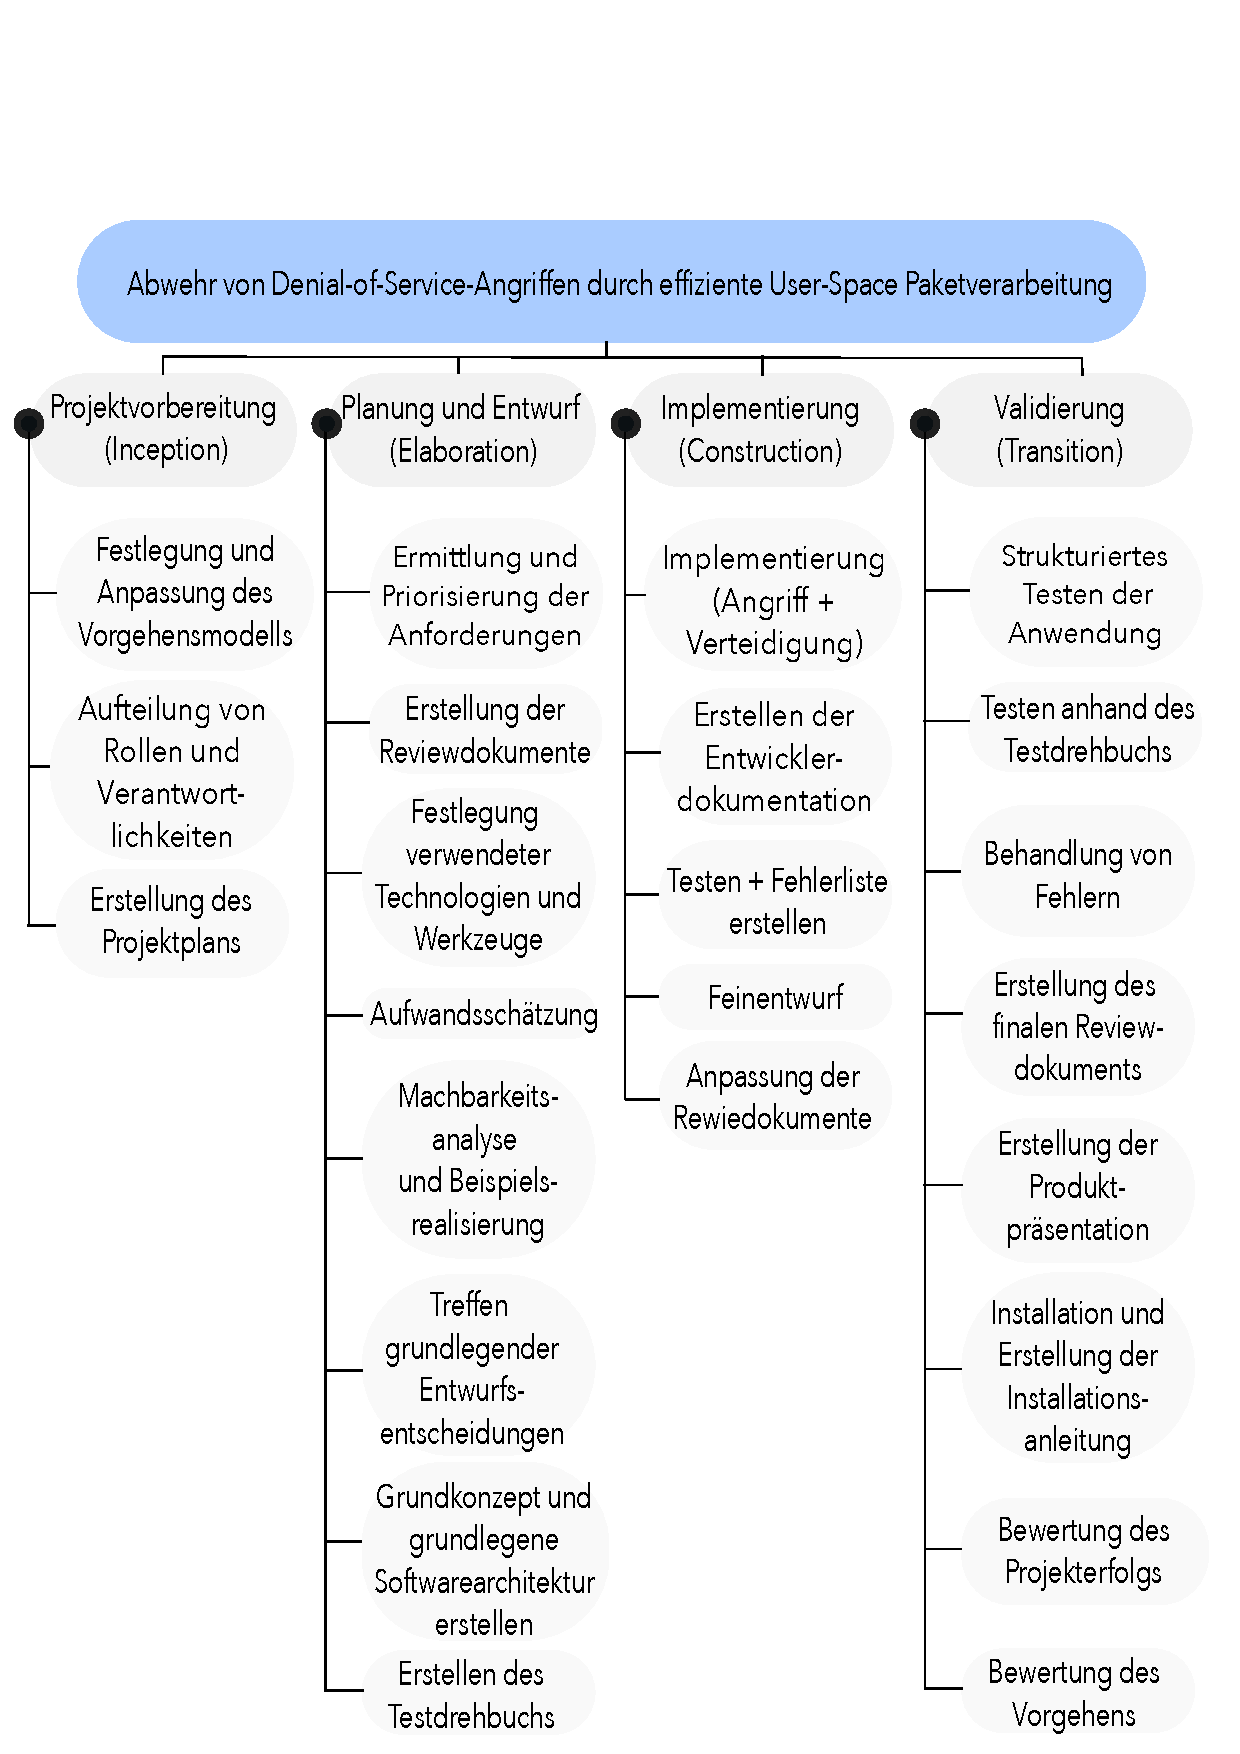
\includegraphics[height = 12.5cm]{projektstrukturplan.pdf}
    \caption{Projektstrukturplan}
    \label{projektstrukturplan}
\end{figure} \\
Der \textbf{Ablaufplan} dient zur zeitlichen Darstellung des Projektablaufes. Die hier gewählte Darstellung ist das Gantt-Diagramm. Mittels Microsoft Project Professional wird so nicht nur das Projekt geplant, gesteuert und überwacht, sondern auch das Gantt-Diagramm erstellt.\\ In den Meetings wird regelmäßig der aktuelle Stand der einzelnen Teammitglieder abgefragt. Somit wird die Werte des Ganntt-Diagramms  kontinuierlich aktualisiert. Die Gantt-Diagramme zu den verschiedenen Phasen sind in den Abbildungen \ref{vm1}, \ref{vm2}, \ref{vm3} und \ref{vm4} zu finden. Dort sind zudem die Abhängigkeiten zwischen den einzelnen Aufgaben zu sehen (zum Beispiel Anfang-zu-Anfang- oder Ende-zu-Anfang-Beziehungen)\\
%MS Project generiert zudem automatisch einen \textbf{Netzplan}, in dem Abhängigkeiten zwischen den einzelnen Teilaufgaben sichtbar werden (vgl. \ref{netzplan}).\\
\begin{figure} [h]
    \centering
    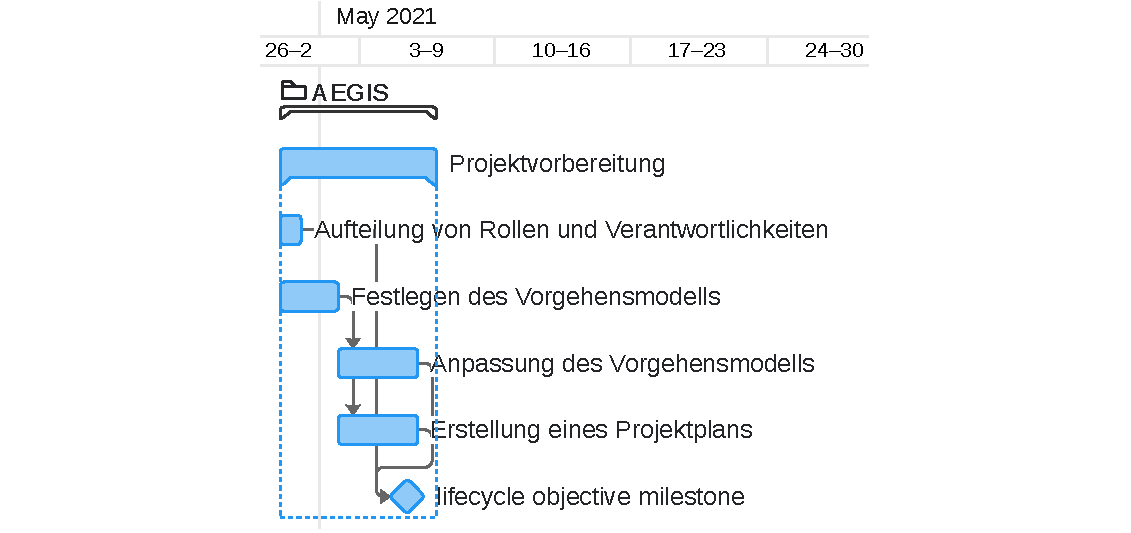
\includegraphics[width=7cm]{gantt_chart_projektvorbereitung.pdf}
    \caption{Ausschnitt des Gantt-Diagramms für die Projektvorbereitungsphase (Stand: 14.05.2021)}     
    \label{vm1}
\end{figure}\\

\begin{figure} [h]
    \centering
    \vspace{-1cm}
    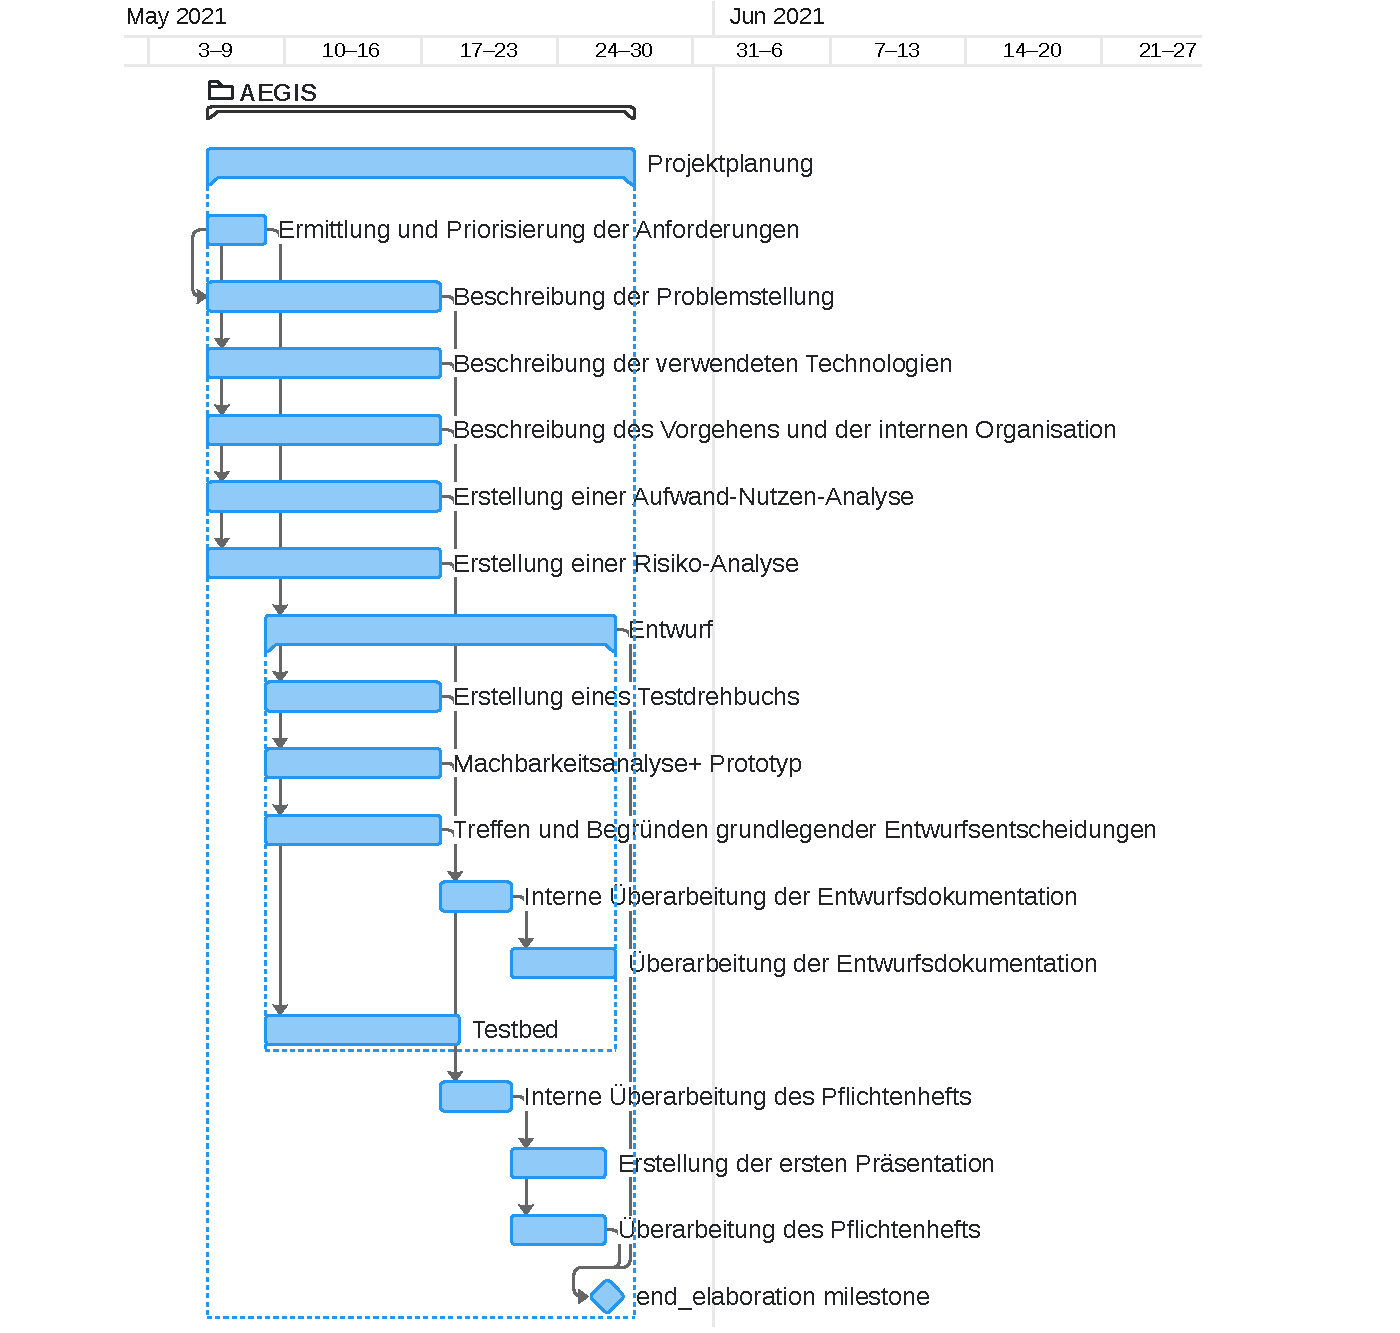
\includegraphics[width=10cm]{gantt_chart_planung_entwurf.pdf}
    \caption{Ausschnitt des Gantt-Diagramms für die Planungs- und Entwurfsphase (Stand: 14.05.2021)}
    \label{vm2}
\end{figure}

\begin{figure} [h]
    \centering
    \vspace{-0.5cm}
    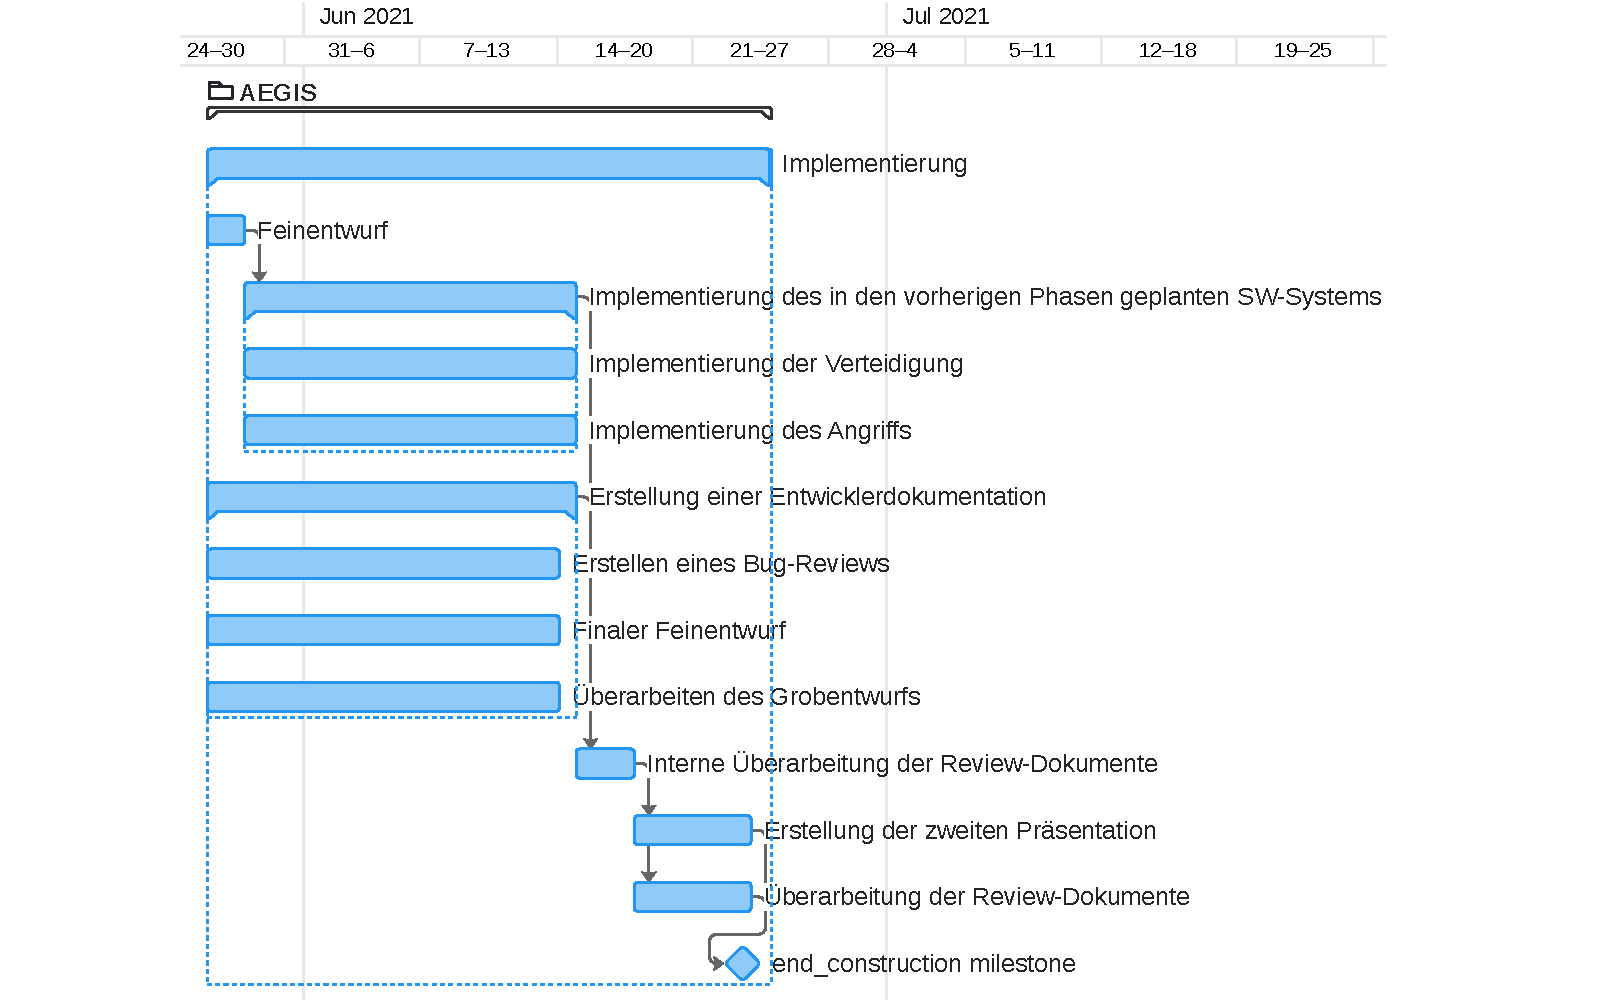
\includegraphics[width=12cm]{gantt_chart_implementierung.pdf}
    \caption{Ausschnitt des Gantt-Diagramms für die Implementierungsphase (Stand: 14.05.2021)}
    \label{vm3}
\end{figure}

\begin{figure} [h]
    \centering
    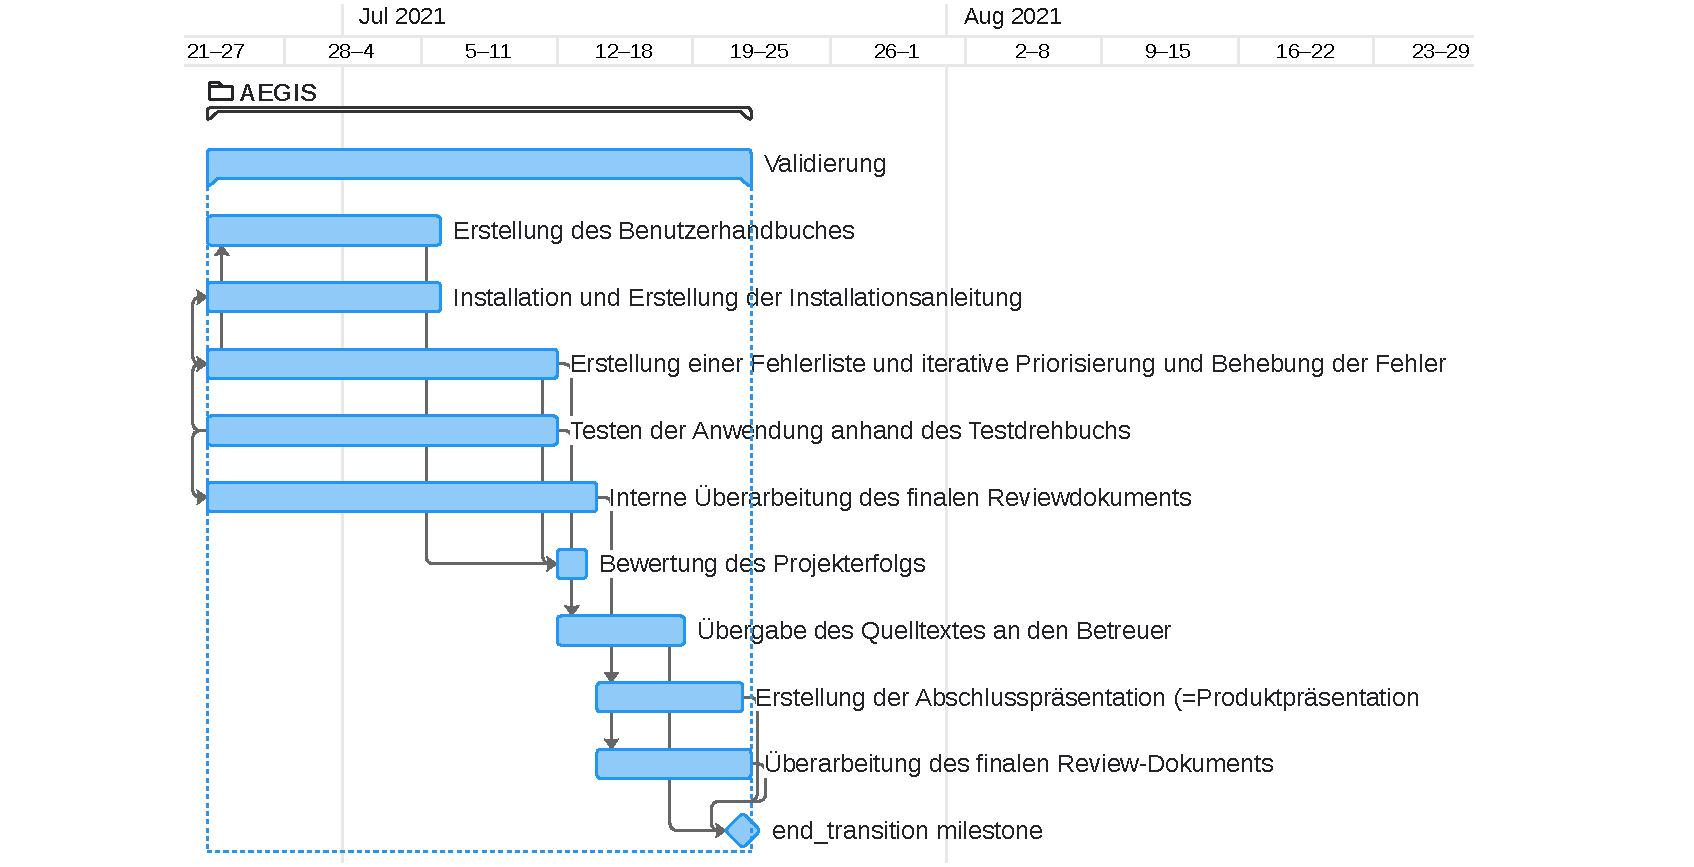
\includegraphics[width=12cm]{gantt_chart_validierung.pdf}
    \caption{Ausschnitt des Gantt-Diagramms für die Validierungssphase (Stand: 14.05.2021)}     
    \label{vm4}
\end{figure}

%\begin{figure} [h]
%    \centering
%    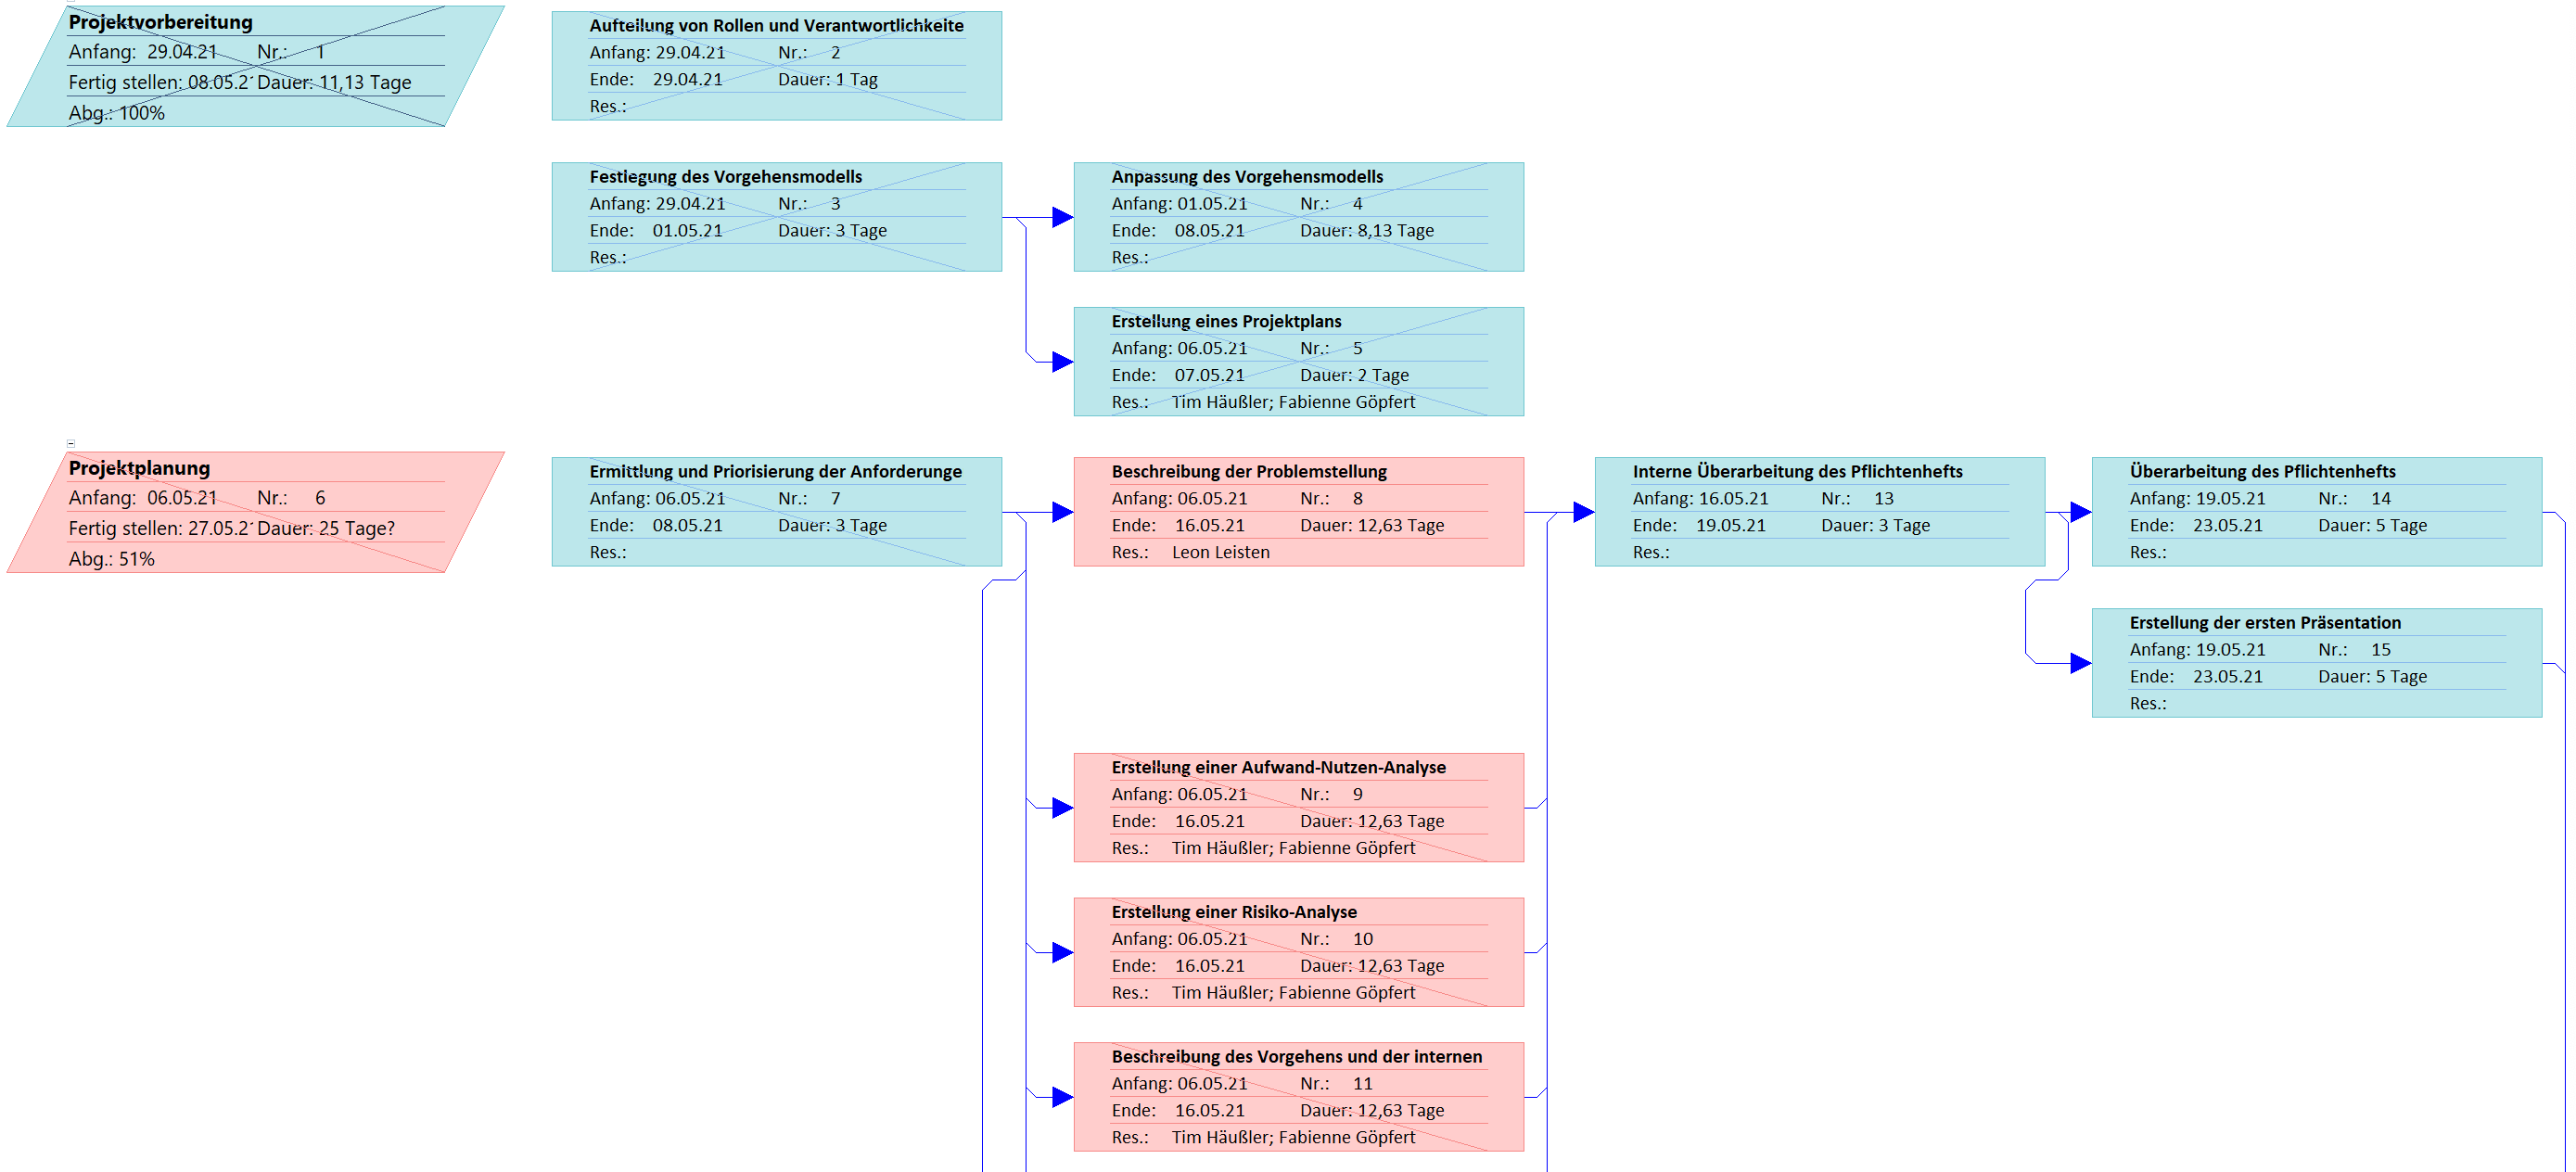
\includegraphics[width=\linewidth, height = 6cm]{netzplan.png}
%    \caption{Ausschnitt des Netzplanes (Stand: 14.05.2021)}
%    \label{netzplan}
%\end{figure}

\section{Meilensteine}
An dieser Stelle kommt zunächst die Frage auf, was ein Meilenstein eigentlich genau ist. Dabei handelt es sich um einen besonders wichtigen Punkt im Projektverlauf, an dem etwas überprüft wird. Ein Meilenstein kann ein Ereignis sein, an dem etwas abgeschlossen ist, etwas begonnen wird oder über die weitere Vorgehensweise entschieden wird.\\
Meilensteine umfassen nie eine Zeitdauer, sondern sind Zeitpunkte und werden meist am Ende von Projektphasen definiert. Es kann allerdings auch innerhalb einzelner Phasen zusätzliche Meilensteine geben.\\
Am 27.05.2021, am 24.06.2021 und am 21.07.2021 finden Reviews für das Softwareprojekt statt, bei denen die Ergebnisse der letzten Phase mit Unterstützung einer Präsentation durch ein oder zwei Studierende vorgestellt werden. Außerdem müssen bis zu diesen drei Tagen die jeweiligen Review-Dokumente fertiggestellt und eingereicht worden sein. Nach der Präsentation und Verteidigung der Ergebnisse werden diese bewertet. Da es sich dabei um Prüfpunkte handelt, stellt ein erfolgreich absolviertes Review die Erreichung eines Meilensteins dar. Außerdem wurde sich passend zum Unified Process für einen Meilenstein am Ende der ersten Konzeptionsphase entschieden.\\
Die vier Meilensteine des hier durchgeführten Projekts sind also die folgenden:
\begin{enumerate}
    \item lifecycle objective
    \item end\_elaboration
    \item end\_construction
    \item end\_transition
\end{enumerate}
Diese sind auch im GitLab erstellt und dein einzelnen Issues zugeordnet. Es bleibt noch anzumerken, dass das Erreichen des letzten Meilensteins gleichzeitig den Projektabschluss darstellt.\\
Außerdem können den drei Projektphasen Elaboration, Construction und Transmission noch jeweils drei Meilensteine mit Bezug zu den Review-Dokumenten zugeordnet werden. Diese sind:
\begin{enumerate}
    \item end\_first\_version
    \item end\_internal\_revision
    \item end\_last\_revision
\end{enumerate}
Damit ist der Abschluss verschiedener Phasen der Erstellung der Review-Dokumente gemeint. Das Ziel lautet bei allen drei Phasen, circa eineinhalb Wochen vor der Abgabe eine erste Fassung erstellt zu haben. Wenn das geschafft wurde, ist der Meilenstein end\_first\_version erreicht. In den darauffolgenden Tagen wird diese Fassung intern, also durch alle Teammitglieder, überarbeitet und verbessert. Dieses überarbeitete Dokument wird dann eine Woche vor der endgültigen Abgabe bei Martin Backhaus eingereicht und der Meilenstein end\_internal\_revision ist erreicht. Schließlich wird in der Woche vor der Abgabe Feedback von Martin Backhaus eingearbeitet und letzte Verbesserungen werden vorgenommen. Mit der Abgabe des Dokuments ist auch der letzte Meilenstein end\_last\_revision erreicht.\\

\end{document}
